\documentclass[aspectratio=169]{beamer}

\usepackage{microtype}
\usepackage{tikzpeople}
\usepackage{drawstack}
\usepackage{graphicx}
\usepackage{fontawesome}
\usepackage{multirow}
\usepackage{fancyvrb}
\usepackage{listings}
\usepackage{siunitx}
\usepackage{tikz}
\usetikzlibrary{calc}
\usetikzlibrary{arrows.meta}
\usetikzlibrary{positioning}
\tikzstyle{block} = [draw, rectangle, 
    minimum height=2em, minimum width=2em]

\newcommand\presdate{June 18, 2020}

\usetheme[]{metropolis}
\metroset{block=fill}

\title{Android: Notifier (Server)}
\date{\presdate}

\author{Marcel Nageler, Sebastian Knoll, Martin Unterguggenberger}
\institute{}

\setbeamertemplate{frame footer}{Android: Notifier (Server) --- Graz, \presdate}

\definecolor{links}{HTML}{2A1B81}
\hypersetup{colorlinks,linkcolor=,urlcolor=links}

\begin{document}
  \maketitle

  \begin{frame}{Content}
    \tableofcontents
  \end{frame}

  %\begin{frame}
  %  \begin{figure}
  %    \centering
  %    \includegraphics[width=\textwidth]{figures/...}
  %    %\caption{}
  %  \end{figure}
  %\end{frame}

\section{Assignment}

  \begin{frame}{Assignment description}
    \begin{block}{Android: Notifier (Server)}
      Receiving notifications from mobile phones on a computer is nothing new (e.g. Messages, Pushbullet, Mightytext, or Desktop Notifications).
      However, all of these services relay your messages using a 3rd party in clear text. Your task is to establish an indirect connection (= using a web server) to a target while ensuring that all transfered data is encrypted. The challenges are similar to the P2P variant. 
      With a server-based version, however, this would also work if the mobile phone and recipient device are located in distinct networks. 
      Somehow you also have to authenticate at the server, i.e. the server has to know the target devices it should deliver notifications for. 
      A very good starting point is in looking at / thinking about how existing messengers, such as Telegram or Signal approach these issues. 
    \end{block}
  \end{frame}

\section{Some Basic Definitions}

  \begin{frame}{Some Basic Definitions}
    The central security properties
    \begin{itemize}
      \item \textbf{Confidentialty} \onslide<1>{$\rightarrow$ Information is not made available to unauthorized entities}
      \pause
      \item \textbf{Integrity} \onslide<2>{$\rightarrow$ Changes can only be done in a specific and authorized manner}
      \pause
      \item \textbf{Availability} \onslide<3>{$\rightarrow$ Timely and reliable access to the information}
      \pause
      \item \textbf{Authencity} \onslide<4>{$\rightarrow$ Assure that information is from the source it claims to be from}
      \pause
    \end{itemize}
    Security properties define what makes assets valuable.
  \end{frame}

\section{Notifications}

  \begin{frame}{Implementation}
    \begin{figure}
      \centering
      \only<1|handout:0>{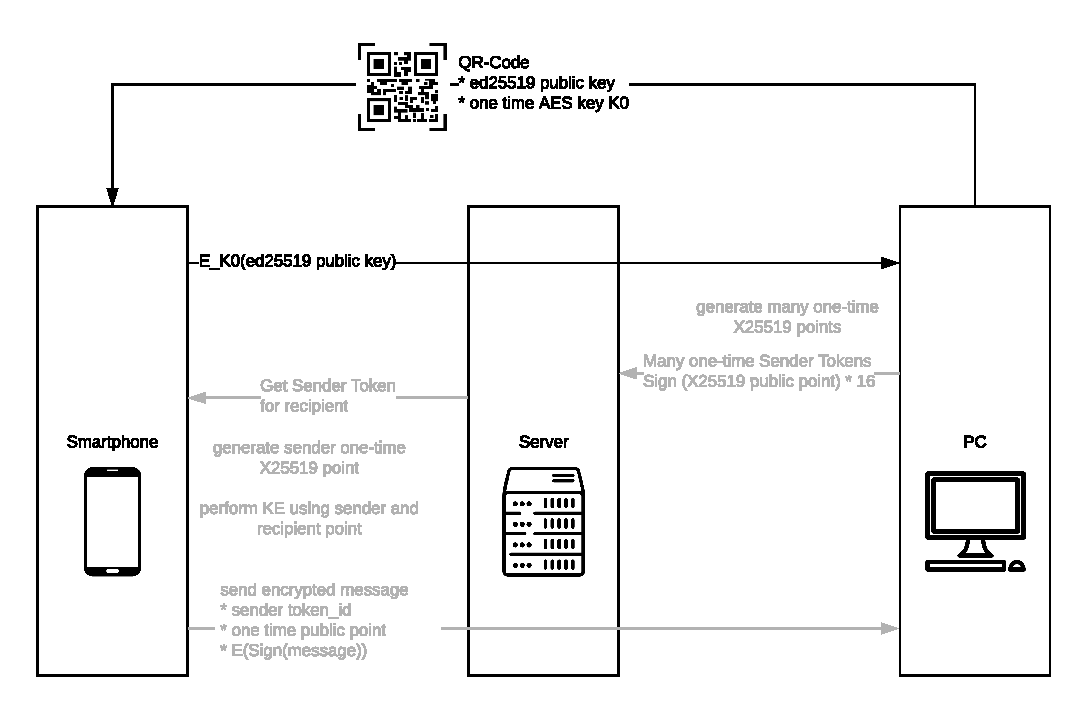
\includegraphics[width=0.7\textwidth]{figures/anim1}}%
      \only<2|handout:0>{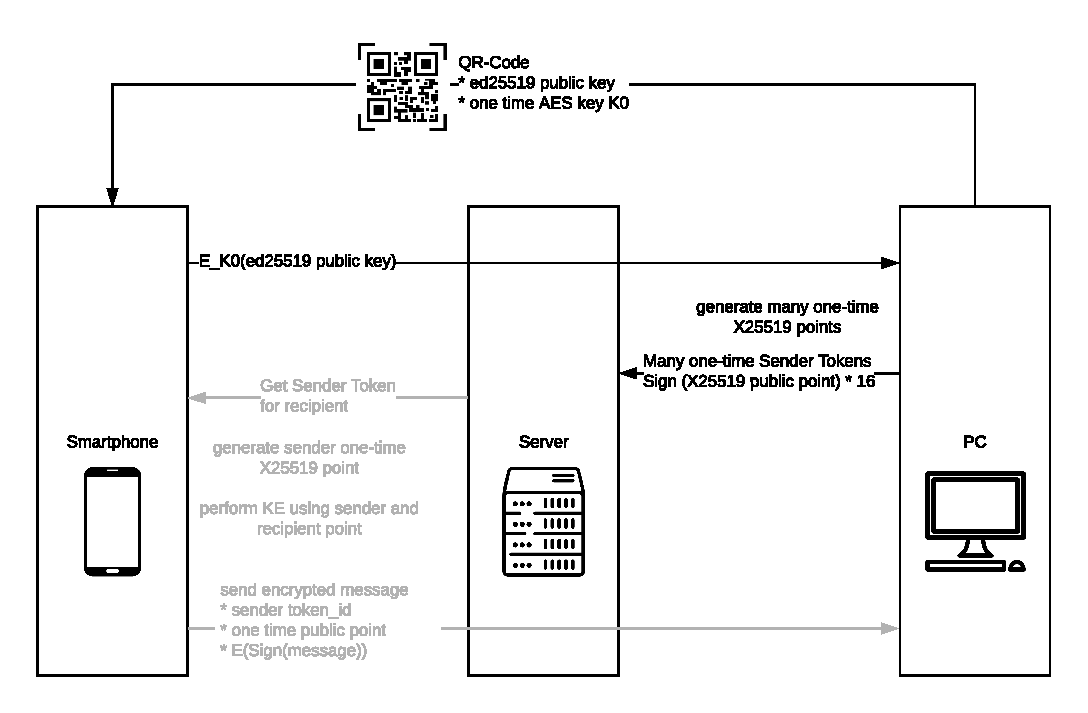
\includegraphics[width=0.7\textwidth]{figures/anim2}}%
      \only<3>{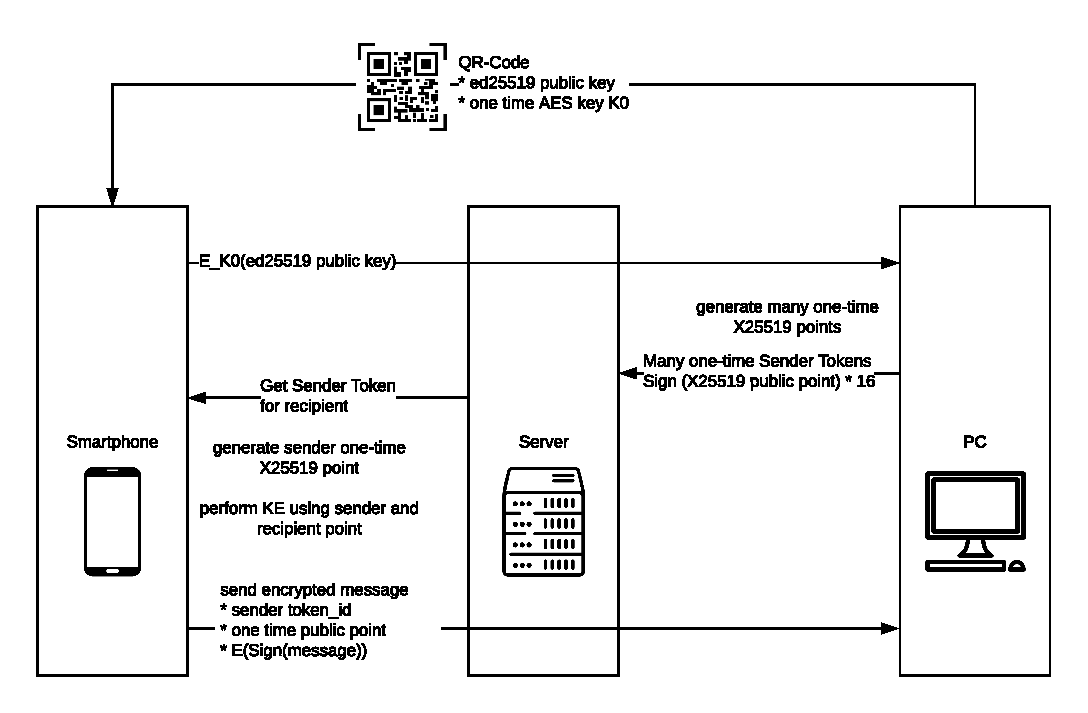
\includegraphics[width=0.7\textwidth]{figures/anim3}}%
      %\caption{}
    \end{figure}
  \end{frame}

  \maketitle
%  \nocite{*}
%  \begin{frame}{References}
%    %\printbibliography
%    \bibliographystyle{alpha}
%    \bibliography{references}
%  \end{frame}
\end{document}
